
\tikzset{every picture/.style={line width=0.75pt}} %set default line width to 0.75pt        

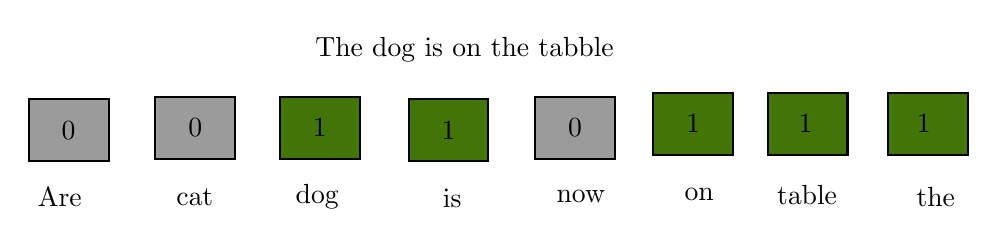
\begin{tikzpicture}[x=0.75pt,y=0.75pt,yscale=-1,xscale=1]
%uncomment if require: \path (0,300); %set diagram left start at 0, and has height of 300

%Shape: Rectangle [id:dp8566339841454302] 
\draw  [fill={rgb, 255:red, 155; green, 155; blue, 155 }  ,fill opacity=1 ] (100,115) -- (138.5,115) -- (138.5,145) -- (100,145) -- cycle ;
%Shape: Rectangle [id:dp35912870192217206] 
\draw  [fill={rgb, 255:red, 155; green, 155; blue, 155 }  ,fill opacity=1 ] (161,114) -- (199.5,114) -- (199.5,144) -- (161,144) -- cycle ;
%Shape: Rectangle [id:dp05913004006588407] 
\draw  [fill={rgb, 255:red, 65; green, 117; blue, 5 }  ,fill opacity=1 ] (221,114) -- (259.5,114) -- (259.5,144) -- (221,144) -- cycle ;
%Shape: Rectangle [id:dp29136466127712035] 
\draw  [fill={rgb, 255:red, 65; green, 117; blue, 5 }  ,fill opacity=1 ] (283,115) -- (321.5,115) -- (321.5,145) -- (283,145) -- cycle ;
%Shape: Rectangle [id:dp3164216751512814] 
\draw  [fill={rgb, 255:red, 155; green, 155; blue, 155 }  ,fill opacity=1 ] (344,114) -- (382.5,114) -- (382.5,144) -- (344,144) -- cycle ;
%Shape: Rectangle [id:dp7942558458095923] 
\draw  [fill={rgb, 255:red, 65; green, 117; blue, 5 }  ,fill opacity=1 ] (401,112) -- (439.5,112) -- (439.5,142) -- (401,142) -- cycle ;
%Shape: Rectangle [id:dp293149550648073] 
\draw  [fill={rgb, 255:red, 65; green, 117; blue, 5 }  ,fill opacity=1 ] (456,112) -- (494.5,112) -- (494.5,142) -- (456,142) -- cycle ;
%Shape: Rectangle [id:dp12157184848090297] 
\draw  [fill={rgb, 255:red, 65; green, 117; blue, 5 }  ,fill opacity=1 ] (514,112) -- (552.5,112) -- (552.5,142) -- (514,142) -- cycle ;

% Text Node
\draw (119.25,130) node  [align=left] {0};
% Text Node
\draw (180.25,129) node  [align=left] {0};
% Text Node
\draw (240.25,129) node  [align=left] {1};
% Text Node
\draw (302.25,130) node  [align=left] {1};
% Text Node
\draw (363.25,129) node  [align=left] {0};
% Text Node
\draw (420.25,127) node  [align=left] {1};
% Text Node
\draw (474.25,127) node  [align=left] {1};
% Text Node
\draw (531.25,127) node  [align=left] {1};
% Text Node
\draw (115,162) node  [align=left] {Are};
% Text Node
\draw (180,162) node  [align=left] {cat};
% Text Node
\draw (239,162) node  [align=left] {dog};
% Text Node
\draw (304,163) node  [align=left] {is};
% Text Node
\draw (366,162) node  [align=left] {now};
% Text Node
\draw (423,161) node  [align=left] {on};
% Text Node
\draw (475,161) node  [align=left] {table};
% Text Node
\draw (537,162) node  [align=left] {the};
% Text Node
\draw (310,91) node  [align=left] {The dog is on the tabble};

\end{tikzpicture}
